% ******************************* PhD Thesis Template **************************
% Please have a look at the README.md file for info on how to use the template

\documentclass[a4paper,12pt,times,numbered,print,index]{Classes/PhDThesisPSnPDF}

% ******************************************************************************
% ******************************* Class Options ********************************
% *********************** See README for more details **************************
% ******************************************************************************

% `a4paper'(The University of Cambridge PhD thesis guidelines recommends a page
% size a4 - default option) or `a5paper': A5 Paper size is also allowed as per
% the Cambridge University Engineering Deparment guidelines for PhD thesis
%
% `11pt' or `12pt'(default): Font Size 10pt is NOT recommended by the University
% guidelines
%
% `oneside' or `twoside'(default): Printing double side (twoside) or single
% side.
%
% `print': Use `print' for print version with appropriate margins and page
% layout. Leaving the options field blank will activate Online version.
%
% `index': For index at the end of the thesis
%
% `draftclassic': For draft mode without loading any images (same as draft in book)
%
% `draft': Special draft mode with line numbers, images, and water mark with
% timestamp and custom text. Position of the text can also be modified.
%
% `abstract': To generate only the title page and abstract page with
% dissertation title and name, to submit to the Student Registry
%
% `chapter`: This option enables only the specified chapter and it's references
%  Useful for review and corrections.
%
% ************************* Custom Page Margins ********************************
%
% `custommargin`: Use `custommargin' in options to activate custom page margins,
% which can be defined in the preamble.tex. Custom margin will override
% print/online margin setup.
%
% *********************** Choosing the Fonts in Class Options ******************
%
% `times' : Times font with math support. (The Cambridge University guidelines
% recommend using times)
%
% `fourier': Utopia Font with Fourier Math font (Font has to be installed)
%            It's a free font.
%
% `customfont': Use `customfont' option in the document class and load the
% package in the preamble.tex
%
% default or leave empty: `Latin Modern' font will be loaded.
%
% ********************** Choosing the Bibliography style ***********************
%
% `authoryear': For author-year citation eg., Krishna (2013)
%
% `numbered': (Default Option) For numbered and sorted citation e.g., [1,5,2]
%
% `custombib': Define your own bibliography style in the `preamble.tex' file.
%              `\RequirePackage[square, sort, numbers, authoryear]{natbib}'.
%              This can be also used to load biblatex instead of natbib
%              (See Preamble)
%
% **************************** Choosing the Page Style *************************
%
% `default (leave empty)': For Page Numbers in Header (Left Even, Right Odd) and
% Chapter Name in Header (Right Even) and Section Name (Left Odd). Blank Footer.
%
% `PageStyleI': Chapter Name next & Page Number on Even Side (Left Even).
% Section Name & Page Number in Header on Odd Side (Right Odd). Footer is empty.
%
% `PageStyleII': Chapter Name on Even Side (Left Even) in Header. Section Number
% and Section Name in Header on Odd Side (Right Odd). Page numbering in footer

% Uncomment to change page style
%\pagestyle{PageStyleII}

% ********************************** Preamble **********************************
% Preamble: Contains packages and user-defined commands and settings
% ******************************************************************************
% ****************************** Custom Margin *********************************

% Add `custommargin' in the document class options to use this section
% Set {innerside margin / outerside margin / topmargin / bottom margin}  and
% other page dimensions
\ifsetCustomMargin
  \RequirePackage[left=37mm,right=30mm,top=35mm,bottom=30mm]{geometry}
  \setFancyHdr % To apply fancy header after geometry package is loaded
\fi

% Add spaces between paragraphs
%\setlength{\parskip}{0.5em}
% Ragged bottom avoids extra whitespaces between paragraphs
\raggedbottom
% To remove the excess top spacing for enumeration, list and description
%\usepackage{enumitem}
%\setlist[enumerate,itemize,description]{topsep=0em}

% *****************************************************************************
% ******************* Fonts (like different typewriter fonts etc.)*************

% Add `customfont' in the document class option to use this section

\ifsetCustomFont
  % Set your custom font here and use `customfont' in options. Leave empty to
  % load computer modern font (default LaTeX font).
  %\RequirePackage{helvet}

  % For use with XeLaTeX
  %  \setmainfont[
  %    Path              = ./libertine/opentype/,
  %    Extension         = .otf,
  %    UprightFont = LinLibertine_R,
  %    BoldFont = LinLibertine_RZ, % Linux Libertine O Regular Semibold
  %    ItalicFont = LinLibertine_RI,
  %    BoldItalicFont = LinLibertine_RZI, % Linux Libertine O Regular Semibold Italic
  %  ]
  %  {libertine}
  %  % load font from system font
  %  \newfontfamily\libertinesystemfont{Linux Libertine O}
\fi

% *****************************************************************************
% **************************** Custom Packages ********************************

% ************************* Algorithms and Pseudocode **************************

%\usepackage{algpseudocode}

% ********************Captions and Hyperreferencing / URL **********************

% Captions: This makes captions of figures use a boldfaced small font.
%\RequirePackage[small,bf]{caption}

\RequirePackage[labelsep=space,tableposition=top]{caption}
\renewcommand{\figurename}{Fig.} %to support older versions of captions.sty


% *************************** Graphics and figures *****************************

%\usepackage{rotating}
%\usepackage{wrapfig}

% Uncomment the following two lines to force Latex to place the figure.
% Use [H] when including graphics. Note 'H' instead of 'h'
%\usepackage{float}
%\restylefloat{figure}

% Subcaption package is also available in the sty folder you can use that by
% uncommenting the following line
% This is for people stuck with older versions of texlive
%\usepackage{sty/caption/subcaption}
\usepackage{subcaption}

% ********************************** Tables ************************************
\usepackage{booktabs} % For professional looking tables
\usepackage{multirow}

%\usepackage{multicol}
%\usepackage{longtable}
%\usepackage{tabularx}


% *********************************** SI Units *********************************
\usepackage{siunitx} % use this package module for SI units


% ******************************* Line Spacing *********************************

% Choose linespacing as appropriate. Default is one-half line spacing as per the
% University guidelines

% \doublespacing
% \onehalfspacing
% \singlespacing


% ************************ Formatting / Footnote *******************************

% Don't break enumeration (etc.) across pages in an ugly manner (default 10000)
%\clubpenalty=500
%\widowpenalty=500

%\usepackage[perpage]{footmisc} %Range of footnote options


% *****************************************************************************
% *************************** Bibliography  and References ********************

%\usepackage{cleveref} %Referencing without need to explicitly state fig /table

% Add `custombib' in the document class option to use this section
\ifuseCustomBib
   \RequirePackage[square, sort, numbers, authoryear]{natbib} % CustomBib

% If you would like to use biblatex for your reference management, as opposed to the default `natbibpackage` pass the option `custombib` in the document class. Comment out the previous line to make sure you don't load the natbib package. Uncomment the following lines and specify the location of references.bib file

%\RequirePackage[backend=biber, style=numeric-comp, citestyle=numeric, sorting=nty, natbib=true]{biblatex}
%\bibliography{References/references} %Location of references.bib only for biblatex

\fi

% changes the default name `Bibliography` -> `References'
\renewcommand{\bibname}{References}


% ******************************************************************************
% ************************* User Defined Commands ******************************
% ******************************************************************************

% *********** To change the name of Table of Contents / LOF and LOT ************

%\renewcommand{\contentsname}{My Table of Contents}
%\renewcommand{\listfigurename}{My List of Figures}
%\renewcommand{\listtablename}{My List of Tables}


% ********************** TOC depth and numbering depth *************************

\setcounter{secnumdepth}{2}
\setcounter{tocdepth}{2}


% ******************************* Nomenclature *********************************

% To change the name of the Nomenclature section, uncomment the following line

%\renewcommand{\nomname}{Symbols}


% ********************************* Appendix ***********************************

% The default value of both \appendixtocname and \appendixpagename is `Appendices'. These names can all be changed via:

%\renewcommand{\appendixtocname}{List of appendices}
%\renewcommand{\appendixname}{Appndx}

% *********************** Configure Draft Mode **********************************

% Uncomment to disable figures in `draft'
%\setkeys{Gin}{draft=true}  % set draft to false to enable figures in `draft'

% These options are active only during the draft mode
% Default text is "Draft"
%\SetDraftText{DRAFT}

% Default Watermark location is top. Location (top/bottom)
%\SetDraftWMPosition{bottom}

% Draft Version - default is v1.0
%\SetDraftVersion{v1.1}

% Draft Text grayscale value (should be between 0-black and 1-white)
% Default value is 0.75
%\SetDraftGrayScale{0.8}


% ******************************** Todo Notes **********************************
%% Uncomment the following lines to have todonotes.

%\ifsetDraft
%	\usepackage[colorinlistoftodos]{todonotes}
%	\newcommand{\mynote}[1]{\todo[author=kks32,size=\small,inline,color=green!40]{#1}}
%\else
%	\newcommand{\mynote}[1]{}
%	\newcommand{\listoftodos}{}
%\fi

% Example todo: \mynote{Hey! I have a note}


% ************************ Thesis Information & Meta-data **********************
% Thesis title and author information, refernce file for biblatex
% ************************ Thesis Information & Meta-data **********************
%% The title of the thesis
\title{Maye Music Backend}
%\texorpdfstring is used for PDF metadata. Usage:
%\texorpdfstring{LaTeX_Version}{PDF Version (non-latex)} eg.,
%\texorpdfstring{$sigma$}{sigma}

%% Subtitle (Optional)
\subtitle{Integracion de plataformas musicales}

%% The full name of the author
\author{
  Echevarria Leandro
  \\[0ex]
  Maquirriain Rodrigo
  \\[0ex]
  Schaerer Daniel
}

%% Department (eg. Department of Engineering, Maths, Physics)
\dept{Departamento de Sistemas}

%% University and Crest
\university{Universidad Tecnológica Nacional}
% Crest minimum should be 30mm.
\crest{
\includegraphics[width=0.2\textwidth]{University_Crest}}
%% Use this crest, if you are using the college crest
%% Crest long miminum should be 65mm
%\crest{
\includegraphics[width=0.45\textwidth]{University_Crest_Long}}

%% College shield [optional] 
% Crest minimum should be 30mm.
%\collegeshield{
\includegraphics[width=0.2\textwidth]{CollegeShields/Kings}}


%% Supervisor (optional)
%% for multiple supervisors, append each supervisor with the \newline command
%\supervisor{Prof. A.B. Supervisor\newline
%Prof. C.D. Supervisor}

%% Supervisor Role (optional) - Supervisor (default) or advisor
% \supervisorrole{\textbf{Supervisors: }}
%% if no title is desired:
% \supervisorrole{}

%% Supervisor line width: required to align supervisors
%\supervisorlinewidth{0.35\textwidth}

%% Advisor (optional)
%% for multiple advisors, append each advisor with the \newline command
%\advisor{Dr. A. Advisor\newline
%Dr. B. Advisor}
     
%% Advisor Role (optional) - Advisor (default) or leave empty
% \advisorrole{Advisors: }
%% if no title is required
% \advisorrole{}

%% Advisor line width: required to align supervisors
%\advisorlinewidth{0.25\textwidth}


%% You can redefine the submission text:
% Default as per the University guidelines:
% ``This dissertation is submitted for the degree of''
%\renewcommand{\submissiontext}{change the default text here if needed}

%% Full title of the Degree
\degreetitle{Técnico Superior en Sistemas Informáticos}

%% College affiliation (optional)
\college{Universidad Tecnológica Nacional}

%% Submission date
% Default is set as {\monthname[\the\month]\space\the\year}
%\degreedate{September 2014} 

%% Meta information
\subject{LaTeX} \keywords{{LaTeX} {PhD Thesis} {Engineering} {University of
Cambridge}}


% ***************************** Abstract Separate ******************************
% To printout only the titlepage and the abstract with the PhD title and the
% author name for submission to the Student Registry, use the `abstract' option in
% the document class.

\ifdefineAbstract
 \pagestyle{empty}
 \includeonly{Declaration/declaration, Abstract/abstract}
\fi

% ***************************** Chapter Mode ***********************************
% The chapter mode allows user to only print particular chapters with references
% Title, Contents, Frontmatter are disabled by default
% Useful option to review a particular chapter or to send it to supervisior.
% To use choose `chapter' option in the document class

\ifdefineChapter
 \includeonly{Chapter3/chapter3}
\fi

% ******************************** Front Matter ********************************
\begin{document}

\frontmatter

\maketitle

% ******************************* Thesis Dedidcation ********************************

\begin{dedication} 

Queremos agradecer a \dots

\end{dedication}
% ******************************* Thesis Declaration ***************************

\begin{declaration}

I hereby declare that except where specific reference is made to the work of 
others, the contents of this dissertation are original and have not been 
submitted in whole or in part for consideration for any other degree or 
qualification in this, or any other university. This dissertation is my own 
work and contains nothing which is the outcome of work done in collaboration 
with others, except as specified in the text and Acknowledgements. This 
dissertation contains fewer than 65,000 words including appendices, 
bibliography, footnotes, tables and equations and has fewer than 150 figures.

% Author and date will be inserted automatically from thesis.tex \author \degreedate

\end{declaration}
% ************************** Thesis Acknowledgements **************************

\begin{acknowledgements}      


And I would like to acknowledge ...


\end{acknowledgements}

% ************************** Thesis Abstract *****************************
% Use `abstract' as an option in the document class to print only the titlepage and the abstract.
\begin{abstract}
This is where you write your abstract ...
\end{abstract}


% *********************** Adding TOC and List of Figures ***********************

\tableofcontents

\listoffigures

\listoftables

% \printnomenclature[space] space can be set as 2em between symbol and description
%\printnomenclature[3em]

\printnomenclature

% ******************************** Main Matter *********************************
\mainmatter

%!TEX root = ../thesis.tex
%*******************************************************************************
%*********************************** First Chapter *****************************
%*******************************************************************************

\chapter{Introducción}  %Title of the First Chapter

\ifpdf
    \graphicspath{{Chapter1/Figs/Raster/}{Chapter1/Figs/PDF/}{Chapter1/Figs/}}
\else
    \graphicspath{{Chapter1/Figs/Vector/}{Chapter1/Figs/}}
\fi


%********************************** %First Section  **************************************
\section{Surgimiento de la musica} %Section - 1.1 

El origen de la música es desconocido, ya que inicialmente no se utilizaban instrumentos
musicales para interpretarla, solo la voz humana, o la percusión corporal, que no dejan
huella en el registro arqueológico. 

Dado que toda cultura conocida ha tenido alguna forma de manifestación musical, la
historia de la música abarca a todas las sociedades y épocas. Se puede inferir que la
música se descubrió en un momento similar a la aparición del lenguaje. El cambio de altura
musical en el lenguaje produce un canto, de manera que es probable que en los orígenes
apareciera de esta manera.

La música de una determinada sociedad está estrechamente relacionada con ciertos aspectos
de su cultura, tales como su organización económica, su desarrollo tecnológico,
tradiciones, creencias religiosas, etcétera. En casi todas las culturas se considera a la
música como un regalo de los dioses. En la Antigua Grecia se consideraba a Hermes como el
transmisor de la música a los humanos, y primer creador de un instrumento musical, el
arpa, al tender cuerdas sobre el caparazón de una tortuga. Hace unos cinco mil años, un
emperador en China, ordenó crear la música a sus súbditos, y les dijo que para ello debían
de basarse en los sonidos de la naturaleza. Entre la mitología germánica se cree que
Heimdall, tenía un cuerno gigantesco que debía tocar cuando comenzara el crepúsculo de los
dioses. Las leyendas son similares para el resto de culturas primitivas, tanto perdidas
como modernas. Al provenir la música, en general, de entidades superiores, habría que
comunicarse con estas entidades también mediante esta música. 

Además, la distinta emotividad a la hora de expresarse, o una expresión rítmica constituye
otra forma de, si no música, sí elementos musicales, como son la interpretación o el
ritmo. Es decir, la música nació al prolongar y elevar los sonidos del lenguaje. 
 
“El arte de la música es el que más cercano se 
halla de las lágrimas y los recuerdos.”
 
En su sentido más amplio, la música nace con el ser humano, y ya estaba presente, es por
tanto una manifestación cultural universal.

La música se podía manifestar en la propia naturaleza o en las actividades cotidianas. Al
golpear dos piedras, o al cortar un árbol, se producía un sonido rítmico, el mantenimiento
de algo rítmico ayudaba a la realización de esa actividad. Pudo haber un primer grito o
palabra que servía como ánimo, apoyo, y para elaborar más eficazmente una determinada
actividad. Estos irían evolucionando a pequeñas frases, versos, hasta terminar ligándolos
en una canción.

\nomenclature[z-cif]{$CIF$}{Cauchy's Integral Formula}                                % first letter Z is for Acronyms 
\nomenclature[a-F]{$F$}{complex function}                                                   % first letter A is for Roman symbols
\nomenclature[g-p]{$\pi$}{ $\simeq 3.14\ldots$}                                             % first letter G is for Greek Symbols
\nomenclature[g-i]{$\iota$}{unit imaginary number $\sqrt{-1}$}                      % first letter G is for Greek Symbols
\nomenclature[g-g]{$\gamma$}{a simply closed curve on a complex plane}  % first letter G is for Greek Symbols
\nomenclature[x-i]{$\oint_\gamma$}{integration around a curve $\gamma$} % first letter X is for Other Symbols
\nomenclature[r-j]{$j$}{superscript index}                                                       % first letter R is for superscripts
\nomenclature[s-0]{$0$}{subscript index}                                                        % first letter S is for subscripts


%********************************** %Second Section  *************************************
\section{Evolución de la música	} %Section - 1.2
\subsection{Prehistoria}

Se desconoce cómo pudo ser la música en la Prehistoria, ya que no queda ningún registro
sonoro ni escrito de la misma. Pero sí que han ido apareciendo pequeños instrumentos, o la
evidencia de cierta tecnología gracias al arte mueble y al arte parietal que permite
pensar el que pudieran haber realizado instrumentos o que tuvieran el desarrollo
suficiente para crear música. A medida que vamos avanzando en el tiempo, vamos encontrando
elementos cada vez más complejos y que no establecen duda alguna de la presencia de
instrumentos en las sociedades prehistóricas y protohistóricas.

Los instrumentos musicales que se encuentran en la Prehistoria se pueden dividir en varios
grupos:
 
Autófonos: aquellos que producen sonidos por medio de la materia con la que están
construidos. Son instrumentos de percusión; por ejemplo, hueso contra piedra.

Membranófonos: serie de instrumentos más sencillos que los construidos por el hombre.

Tambores: hechos con una membrana tirante, sobre una nuez de coco, un recipiente
cualquiera o una verdadera y auténtica caja de resonancia.

Cordófonos: son aquellos de cuerda; por ejemplo, el arpa.

Aerófonos: el sonido se origina en ellos por vibraciones de una columna de aire. Uno de
los primeros instrumentos es la flauta, en un principio construida con un hueso con
agujeros.


\subsection{Paleolítico}

En el Paleolítico superior y más raramente en el Paleolítico Medio es donde encontramos
evidencias o indicios de la existencia tanto de primitivos instrumentos musicales como de
representaciones artísticas de los mismos. Desde finales del siglo XIX se viene publicando
la presencia de pitos o flautas encontradas en diversos yacimientos, pero solamente han
empezado a ser tomadas en serio y estudiadas en profundidad desde los años 60 del siglo
XX, en la actualidad, este sigue siendo un campo bastante polémico. Por un lado, hay
discusiones abiertas sobre si ciertos instrumentos estaban hechos para producir sonido, y
por otro lado si en realidad tienen un origen antrópico o son por el contrario el
resultado de depredadores y la erosión.


\subsection{Neolítico}

Escena de caza, en el Barranco de la Valltorta. Se aprecian los arcos y las cuerdas.

Tenemos muchos ejemplos en la pintura rupestre del periodo Neolítico de la existencia de
arcos. Aunque la mayoría se encuentran en contextos de caza, la realidad es que si
conocían la manera de construir un arco también sabían que una cuerda tensada a distintas
longitudes produce sonidos distintos.


\subsection{Antiguo Egipto y Mesopotamia}

La música en Egipto poseía avanzados conocimientos que eran reservados para los
sacerdotes. En el Imperio Nuevo utilizaban ya la escala de siete sonidos. Este pueblo
contó con un instrumentario rico y variado; algunos de los más representativos son el arpa
como instrumento de cuerdas y el oboe doble como instrumento de viento. En Mesopotamia los
músicos eran considerados personas de gran prestigio; acompañaban al monarca no solo en
los actos de culto, sino también en las suntuosas ceremonias de palacio y en las guerras.
El arpa es uno de los instrumentos más apreciados en Mesopotamia. La expresión musical de 
la Mesopotamia es considerada origen de la cultura musical occidental.


\subsection{Antigua Grecia}

En la Antigua Grecia, la música se vio influida por todas las civilizaciones que la
rodeaban, dada su importante posición estratégica. Culturas como la mesopotámica, etrusca,
egipcia o incluso las indoeuropeas fueron de importante influencia tanto en sus músicas
como en sus instrumentos musicales. Los griegos daban mucha importancia al valor educativo
y moral de la música. Por ello está muy relacionada con el poema épico. Aparecen los
bardos o aedos que, acompañados de una lira, vagan de pueblo en pueblo mendigando y
guardando memoria oral de la historia de Grecia y sus leyendas. Fue entonces cuando se
relaciona la música estrechamente con la filosofía. Los sabios de la época resaltan el
valor cultural de la música.


\subsection{Antigua Roma}

Habitualmente se utilizaba la música en las grandes fiestas. Eran muy valorados los
músicos virtuosos o famosos, añadiendo vertientes humorísticas y distendidas a sus
actuaciones. Estos músicos vivían de una manera bohemia, rodeados siempre de fiestas.

En los teatros romanos o anfiteatros se representaban comedias al estilo griego. La música
tenía un papel trascendental en estas obras teatrales.

A partir de la fundación de Roma sucede un hito musical, los ludiones. Estos eran unos
actores de origen etrusco que bailaban al ritmo de la tibia (una especie de instrumento
musical de viento). Los romanos intentan imitar estos artes y añaden el elemento de la
música vocal. A estos nuevos artistas se les denominó histriones que significa bailarines
en etrusco. Ninguna música de este estilo ha llegado hasta nosotros salvo un pequeño
fragmento de una comedia de Terencio.


\subsection{Edad Media}

Los orígenes de la música medieval se confunden con los últimos desarrollos de la música
del periodo tardío romano. La evolución de las formas musicales apegadas al culto se
resolvió a finales del siglo VI en el llamado canto gregoriano (se refiere en general a un
tipo de canto llano utilizado en la liturgia de la Iglesia católica, aunque en ocasiones
se usa en un sentido amplio o incluso como sinónimo de canto llano).


\subsection{Renacimiento}

Se caracteriza por una suave sonoridad que deriva de la aceptación de la tercera como
intervalo armónico consonante (uniéndose en esta categoría a quintas y octavas, ya
 admitidas en la Edad Media) y del progresivo aumento del número de voces, todas de igual
 importancia y regidas por las reglas del contrapunto: independencia de las voces,
 preparación y resolución de las disonancias, uso de terceras y sextas paralelas,
 exclusión de las quintas y octavas paralelas, etcétera.

El prototipo de obra musical renacentista es una pieza vocal de textura polifónica,
frecuentemente imitativa, escrita para entre tres y seis voces de carácter cantable; cada
línea melódica o voz podía ser interpretada indistintamente con voces reales o con
instrumentos. Si bien el rango de cada línea supera apenas la octava, la extensión general
del conjunto rebasa ampliamente las dos octavas, evitándose el cruce entre las voces (que
forzaba a que estas fueran heterogéneas y contrastantes en la polifonía medieval).

El sistema melódico utilizado siguió siendo el de los ocho modos gregorianos; las
características modales (opuestas a las tonales) de la música del Renacimiento comenzaron
a diluirse hacia el final del período con el uso creciente de intervalos de quinta como
movimiento entre fundamentales, característica definitoria de la tonalidad.


\subsection{Período de la práctica común o clásica}

En este período se desarrollaron nuevas formas y se operaron grandes avances técnicos
tanto en la composición como en el virtuosismo; así tenemos: cromatismo, expresividad,
bajo cifrado y bajo continuo, intensidad, ópera, oratorio, cantata, sonata, tocata, suite,
fuga y la sinfonía.


\subsection{Bajo contínuo}

También llamado bajo cifrado, permitía al compositor trazar tan solo el contorno de la
melodía  dejando las voces medias, es decir, el relleno armónico, a la invención del
continuista. La ejecución del continuo requiere dos instrumentistas: un instrumento
melódico grave (viola, gamba, violonchelo, contrabajo, fagot, etc.) que ejecuta las notas
del bajo y un instrumento armónico (laúd, clavecín, órgano) a cargo del continuista, quien
 desenvuelve improvisadamente las armonías, de acuerdo con las cifras del bajo cifrado, en
 la forma de acordes arpegios u otras figuraciones, todo ello de conforme al estilo y las
 necesidades expresivas del texto musical.


\subsection{Sistema tonal}

El sistema tonal fue una evolución desde los últimos maestros de la música medieval hasta
su máximo esplendor desde Bach a los últimos compositores tonales del posromanticismo. En
sus comienzos, se definió una armonía musical compuesta por siete asuntos distintos: Las
notas, los intervalos, los géneros, los sistemas de escala, los tonos, la modulación y la
composición de melodías.


\subsection{Clasicismo}

Es el estilo caracterizado por la transición de la música barroca hacia una música
equilibrada entre estructura y melodía. Ocupa la segunda mitad del siglo XVIII. Autores
que han marcado historia en este periodo fueron Carl Philipp Emanuel Bach, Franz Joseph
Haydn, Wolfgang Amadeus Mozart y Ludwig van Beethoven. 


\subsection{Romanticismo}

Aproximadamente desde 1830, lo romántico hace su aparición en toda Europa. Ha sido un
fenómeno que se fue instalando con el paso del tiempo. Se dice que en las últimas obras
de Mozart se puede apreciar algo de pre romanticismo.

El romanticismo es un movimiento que se inserta en todos los planos de la vida. Se 
caracteriza por el sentimiento, la pasión, imaginación, dominio del corazón sobre la 
cabeza y por el sentido de libertad.

La música romántica es apasionada, con frecuencia busca sonidos horrísonos para expresar
los más tremendos sentimientos


\subsection{Impresionismo}

La corriente dominante en Europa, influida por la mentalidad positivista, era ya el
realismo.

El impresionismo trata de representar no toda la realidad, sino lo que nos llama la
atención de la realidad, las sensaciones que nos produce. 

Los músicos llegaron un poco más tarde a este período pero también han encontrado una
manera de expresarse musicalmente. Buscaron sonidos líquidos, tímidos, decadentes,
calurosos. Buscaban sugerir cosas al público, darles un primer vistazo de lo que el músico
buscaba producir en su público.


\subsection{Contemporáneo}

Durante el siglo XX, sobre todo en la primera mitad, se ha ido perdiendo la relación entre 
los compositores y los inventores. Una de las posibles causas de la pérdida de esta
relación es que la música del siglo XX es poco comercial. La investigación por hallar
sonidos distintos es poco rentable.

Los nuevos sonidos, que los compositores necesitan para expresar lo que desean han
acabado obteniéndose no de instrumentos manuales, sino por medios electrónicos, hoy día
más al alcance de un músico que de los aparatos mecánicos. La nueva música tenía que
buscar su forma de expresión, y es el campo de la electrónica aquel en que se ha tratado
de encontrar la respuesta (no debemos confundir esto con el propio género de música
electrónica).


\nomenclature[z-DEM]{DEM}{Discrete Element Method}
\nomenclature[z-FEM]{FEM}{Finite Element Method}
\nomenclature[z-PFEM]{PFEM}{Particle Finite Element Method}
\nomenclature[z-FVM]{FVM}{Finite Volume Method}
\nomenclature[z-BEM]{BEM}{Boundary Element Method}
\nomenclature[z-MPM]{MPM}{Material Point Method}
\nomenclature[z-LBM]{LBM}{Lattice Boltzmann Method}
\nomenclature[z-MRT]{MRT}{Multi-Relaxation 
Time}
\nomenclature[z-RVE]{RVE}{Representative Elemental Volume}
\nomenclature[z-GPU]{GPU}{Graphics Processing Unit}
\nomenclature[z-SH]{SH}{Savage Hutter}
\nomenclature[z-CFD]{CFD}{Computational Fluid Dynamics}
\nomenclature[z-LES]{LES}{Large Eddy Simulation}
\nomenclature[z-FLOP]{FLOP}{Floating Point Operations}
\nomenclature[z-ALU]{ALU}{Arithmetic Logic Unit}
\nomenclature[z-FPU]{FPU}{Floating Point Unit}
\nomenclature[z-SM]{SM}{Streaming Multiprocessors}
\nomenclature[z-PCI]{PCI}{Peripheral Component Interconnect}
\nomenclature[z-CK]{CK}{Carman - Kozeny}
\nomenclature[z-CD]{CD}{Contact Dynamics}
\nomenclature[z-DNS]{DNS}{Direct Numerical Simulation}
\nomenclature[z-EFG]{EFG}{Element-Free Galerkin}
\nomenclature[z-PIC]{PIC}{Particle-in-cell}
\nomenclature[z-USF]{USF}{Update Stress First}
\nomenclature[z-USL]{USL}{Update Stress Last}
\nomenclature[s-crit]{crit}{Critical state}
\nomenclature[z-DKT]{DKT}{Draft Kiss Tumble}
\nomenclature[z-PPC]{PPC}{Particles per cell}
%!TEX root = ../thesis.tex
%*******************************************************************************
%****************************** Second Chapter *********************************
%*******************************************************************************

\chapter{Marco teórico}

\ifpdf
    \graphicspath{{Chapter2/Figs/Raster/}{Chapter2/Figs/PDF/}{Chapter2/Figs/}}
\else
    \graphicspath{{Chapter2/Figs/Vector/}{Chapter2/Figs/}}
\fi


\section{Tecnologías}

\subsection{HTTP}

HTTP, Hypertext Transfer Protocol (Protocolo de Transferencia de Hipertexto) por sus
siglas, es el protocolo por el cual se comunican navegadores, servidores y aplicaciones
relacionadas con la web alrededor de todo el mundo.

Este protocolo se encuentra en la capa de aplicación del modelo OSI. Ha estado en uso por
la World-Wide Web (WWW) desde 1990. Su primera versión hace referencia a HTTP/0.9 y era un 
protocolo simple para la transferencia de datos a través de la internet.

HTTP/1.0 surge a través de la definición del RFC 1945, este mejoró sustancialmente la
comunicación permitiendo a los mensajes encontrarse en formato MIME (Multipurpose
Internet Mail Extensions). Los servidores web adjuntan un tipo MIME a todas sus peticiones
HTTP. Cuando un navegador web obtiene una respuesta desde un servidor, mira el tipo MIME
asociado a ella para ver si sabe cómo manejar el archivo. La mayoría de los navegadores
pueden manejar cientos de tipos de archivos populares: Imágenes, videos, sonidos,
documentos de texto, entre otros.

La última versión de este procolo es la 2.0, definida en el RFC 7540 en el año 2015. Un
gran avance en esta última versión contribuye a disminuir el tráfico innecesario en 
la red definiendo un mapeo optimizado de la semántica de HTTP a una conexión subyacente.

El modo de funcionamiento es muy sencillo. Esta compuesto por dos partes quienes son 
las partes que se comunican, estas son el cliente y el servidor. Básicamente el cliente
envía peticiones al servidor y este debe servirlas en caso de poder. De lo contrario, 
el servidor devolverá el error correspondiente a alguna de las posibles causas. Algunas 
de las más comunes son que el recurso que el servidor busca no se encuentre, que el 
recurso no esté disponible, que se haya movido de lugar o que haya habido algún error 
interno.

\begin{figure}[htbp!] 
\centering    
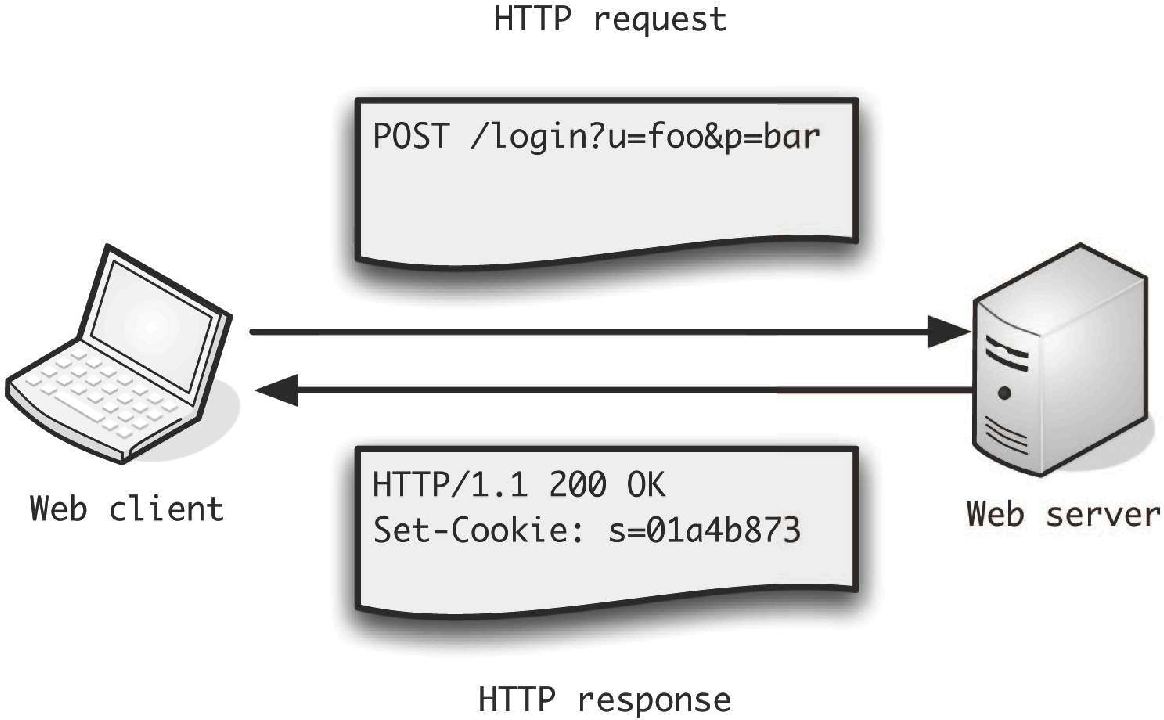
\includegraphics[width=0.5\textwidth]{http1}
\caption[HTTP]{Este es el comportamiento con información básica del protocolo HTTP}
\label{fig:http-behavior}
\end{figure}


\subsection{API REST}

La sigla REST responde a Representational State Transfer- Transferencia de Estado
Representacional. Es cualquier interfaz entre sistemas que use HTTP para obtener
datos o generar operaciones sobre esos datos en todos los formatos posibles, como XML y
JSON. También podemos decir que es un estilo de arquitectura para proveer estándares entre
sistemas de computadoras en la web. 

Su creador, Roy Fielding, es también coautor del protocolo HTTP mencionado en el capítulo 
anterior. REST nace en el año 2000.

La arquitectura REST describe seis restricciones que definen la base del estilo 
RESTful:

\begin{itemize}
   \item first item
   \begin{itemize}
     \item first nested item
     \item second nested item
   \end{itemize}
   \item second item
   \item third item
\end{itemize}


\begin{itemize}
   \item Interfaz Uniforme
	
	Define la interfaz entre clientes y servidores. Simplifica y desacopla la 
	arquitectura. Tiene cuatro principios:
	   
   \begin{itemize}
     \item Basada en Recursos
     
	Los recursos son identificados individualmente en las peticiones usando su URI como
	identificadores. Los recursos en si mismos están separados de lo que terminará siendo 
	su representación devuelta al cliente.     
     
     \item Manipulación de recursos a través de representaciones
     
     Cuando un cliente tiene una representación de algún recurso, esto es suficiente 
     para modificar o eliminar el recurso siempre y cuando se tenga permiso para esto.
     
     \item Mensajes auto descriptivos
     
     Cada mensaje incluye suficiente información describiendo cómo debe éste procesarse.
     
     \item Hypermedia as the Engine of Application State (HATEOAS)
     
     Los clientes entregan el estado a través del contenido del body, los parámetros de
     la query, los headers del request y el URI solicitado (el nombre del recurso). 
     Los servicios entregan estado a los clientes a través del
     body, códigos de respuesta y headers en la respuesta.
   \end{itemize}
   
	\item Sin estado
	
	Esto significa que el estado necesario para manejar la petición está contenido en 
	la petición en si misma como parte de la URI, los parámetros de la query, el body o 
	los headers. La URI identifica de manera única al recurso y el body contiene el estado 
	(o el cambio de éste) de ese recurso. Luego de que el servidor procese lo necesario, 
	la información pertinente es devuelta al cliente mediante headers, estados y el body.
	
	\item Cacheable
	
	Los clientes pueden cachear respuestas. Las respuestas deben definirse a si mismas 
	como cacheables o no cacheables. Esto es para evitar que los clientes reutilicen datos 
	inapropiados u obsoletos.
	
	\item Cliente-Servidor 
	
	La interfaz uniforme separa los clientes de los servidores. Esta separación de 
	conceptos significa que, por ejemplo, los clientes no están envueltos en el guardado 
	de datos, tarea que recae internamente en cada servidor. Por otro lado, los servidores
	no se preocupan por la interfaz de usuario o por el estado de éste. Mientras la 
	interfaz se mantenga, tanto cliente como servidor pueden ser desarrollados y/o 
	reemplazados.
	
	\item Sistema en capas
	
	Un cliente no posee la capacidad por si mismo de decir si está conectado al 
	servidor final o a un servidor intermedio. Los servidores intermedios pueden aumentar 
	la escalabilidad activando balanceadores de carga o caches compartidos.
	
	\item Código en demanda (opcional)
	
	Los servidores son temporalmente capaces de transferir al cliente funcionalidades o 
	código que éstos puedan ejecutar.

\end{itemize}

 
\subsection{AJAX}

\subsection{JWT}

\subsection{Memoria Cache}


\section{Herramientas y tecnologías utilizadas}

\subsection{PHP}

\subsection{Lumen Framework}

\subsection{SQL}

\subsection{Taiga}

\subsection{Vagrant}

\subsection{Git}
%!TEX root = ../thesis.tex
%*******************************************************************************
%****************************** Third Chapter **********************************
%*******************************************************************************
\chapter{My third chapter}

% **************************** Define Graphics Path **************************
\ifpdf
    \graphicspath{{Chapter3/Figs/Raster/}{Chapter3/Figs/PDF/}{Chapter3/Figs/}}
\else
    \graphicspath{{Chapter3/Figs/Vector/}{Chapter3/Figs/}}
\fi

\section{First section of the third chapter}
And now I begin my third chapter here \dots

And now to cite some more people~\citet{Rea85,Ancey1996}

\subsection{First subsection in the first section}
\dots and some more 

\subsection{Second subsection in the first section}
\dots and some more \dots

\subsubsection{First subsub section in the second subsection}
\dots and some more in the first subsub section otherwise it all looks the same
doesn't it? well we can add some text to it \dots

\subsection{Third subsection in the first section}
\dots and some more \dots

\subsubsection{First subsub section in the third subsection}
\dots and some more in the first subsub section otherwise it all looks the same
doesn't it? well we can add some text to it and some more and some more and
some more and some more and some more and some more and some more \dots

\subsubsection{Second subsub section in the third subsection}
\dots and some more in the first subsub section otherwise it all looks the same
doesn't it? well we can add some text to it \dots

\section{Second section of the third chapter}
and here I write more \dots

\section{The layout of formal tables}
This section has been modified from ``Publication quality tables in \LaTeX*''
 by Simon Fear.

The layout of a table has been established over centuries of experience and 
should only be altered in extraordinary circumstances. 

When formatting a table, remember two simple guidelines at all times:

\begin{enumerate}
  \item Never, ever use vertical rules (lines).
  \item Never use double rules.
\end{enumerate}

These guidelines may seem extreme but I have
never found a good argument in favour of breaking them. For
example, if you feel that the information in the left half of
a table is so different from that on the right that it needs
to be separated by a vertical line, then you should use two
tables instead. Not everyone follows the second guideline:

There are three further guidelines worth mentioning here as they
are generally not known outside the circle of professional
typesetters and subeditors:

\begin{enumerate}\setcounter{enumi}{2}
  \item Put the units in the column heading (not in the body of
          the table).
  \item Always precede a decimal point by a digit; thus 0.1
      {\em not} just .1.
  \item Do not use `ditto' signs or any other such convention to
      repeat a previous value. In many circumstances a blank
      will serve just as well. If it won't, then repeat the value.
\end{enumerate}

A frequently seen mistake is to use `\textbackslash begin\{center\}' \dots `\textbackslash end\{center\}' inside a figure or table environment. This center environment can cause additional vertical space. If you want to avoid that just use `\textbackslash centering'


\begin{table}
\caption{A badly formatted table}
\centering
\label{table:bad_table}
\begin{tabular}{|l|c|c|c|c|}
\hline 
& \multicolumn{2}{c}{Species I} & \multicolumn{2}{c|}{Species II} \\ 
\hline
Dental measurement  & mean & SD  & mean & SD  \\ \hline 
\hline
I1MD & 6.23 & 0.91 & 5.2  & 0.7  \\
\hline 
I1LL & 7.48 & 0.56 & 8.7  & 0.71 \\
\hline 
I2MD & 3.99 & 0.63 & 4.22 & 0.54 \\
\hline 
I2LL & 6.81 & 0.02 & 6.66 & 0.01 \\
\hline 
CMD & 13.47 & 0.09 & 10.55 & 0.05 \\
\hline 
CBL & 11.88 & 0.05 & 13.11 & 0.04\\ 
\hline 
\end{tabular}
\end{table}

\begin{table}
\caption{A nice looking table}
\centering
\label{table:nice_table}
\begin{tabular}{l c c c c}
\hline 
\multirow{2}{*}{Dental measurement} & \multicolumn{2}{c}{Species I} & \multicolumn{2}{c}{Species II} \\ 
\cline{2-5}
  & mean & SD  & mean & SD  \\ 
\hline
I1MD & 6.23 & 0.91 & 5.2  & 0.7  \\

I1LL & 7.48 & 0.56 & 8.7  & 0.71 \\

I2MD & 3.99 & 0.63 & 4.22 & 0.54 \\

I2LL & 6.81 & 0.02 & 6.66 & 0.01 \\

CMD & 13.47 & 0.09 & 10.55 & 0.05 \\

CBL & 11.88 & 0.05 & 13.11 & 0.04\\ 
\hline 
\end{tabular}
\end{table}


\begin{table}
\caption{Even better looking table using booktabs}
\centering
\label{table:good_table}
\begin{tabular}{l c c c c}
\toprule
\multirow{2}{*}{Dental measurement} & \multicolumn{2}{c}{Species I} & \multicolumn{2}{c}{Species II} \\ 
\cmidrule{2-5}
  & mean & SD  & mean & SD  \\ 
\midrule
I1MD & 6.23 & 0.91 & 5.2  & 0.7  \\

I1LL & 7.48 & 0.56 & 8.7  & 0.71 \\

I2MD & 3.99 & 0.63 & 4.22 & 0.54 \\

I2LL & 6.81 & 0.02 & 6.66 & 0.01 \\

CMD & 13.47 & 0.09 & 10.55 & 0.05 \\

CBL & 11.88 & 0.05 & 13.11 & 0.04\\ 
\bottomrule
\end{tabular}
\end{table}

%\include{Chapter4/chapter4}
%\include{Chapter5/chapter5}
%\include{Chapter6/chapter6}
%\include{Chapter7/chapter7}



% ********************************** Back Matter *******************************
% Backmatter should be commented out, if you are using appendices after References
%\backmatter

% ********************************** Bibliography ******************************
\begin{spacing}{0.9}

% To use the conventional natbib style referencing
% Bibliography style previews: http://nodonn.tipido.net/bibstyle.php
% Reference styles: http://sites.stat.psu.edu/~surajit/present/bib.htm

\bibliographystyle{apalike}
%\bibliographystyle{unsrt} % Use for unsorted references  
%\bibliographystyle{plainnat} % use this to have URLs listed in References
\cleardoublepage
\bibliography{References/references} % Path to your References.bib file


% If you would like to use BibLaTeX for your references, pass `custombib' as
% an option in the document class. The location of 'reference.bib' should be
% specified in the preamble.tex file in the custombib section.
% Comment out the lines related to natbib above and uncomment the following line.

%\printbibliography[heading=bibintoc, title={References}]


\end{spacing}

% ********************************** Appendices ********************************

\begin{appendices} % Using appendices environment for more functunality

%!TEX root = ../thesis.tex
% ******************************* Thesis Appendix A ****************************
\chapter{How to install \LaTeX} 

\section*{Windows OS}

\subsection*{TeXLive package - full version}
\begin{enumerate}
\item	Download the TeXLive ISO (2.2GB) from\\
\href{https://www.tug.org/texlive/}{https://www.tug.org/texlive/}
\item	Download WinCDEmu (if you don't have a virtual drive) from \\
\href{http://wincdemu.sysprogs.org/download/}
{http://wincdemu.sysprogs.org/download/}
\item	To install Windows CD Emulator follow the instructions at\\
\href{http://wincdemu.sysprogs.org/tutorials/install/}
{http://wincdemu.sysprogs.org/tutorials/install/}
\item	Right click the iso and mount it using the WinCDEmu as shown in \\
\href{http://wincdemu.sysprogs.org/tutorials/mount/}{
http://wincdemu.sysprogs.org/tutorials/mount/}
\item	Open your virtual drive and run setup.pl
\end{enumerate}

or

\subsection*{Basic MikTeX - \TeX~ distribution}
\begin{enumerate}
\item	Download Basic-MiK\TeX (32bit or 64bit) from\\
\href{http://miktex.org/download}{http://miktex.org/download}
\item	Run the installer 
\item	To add a new package go to Start >> All Programs >> MikTex >> Maintenance (Admin) and choose Package Manager
\item	Select or search for packages to install
\end{enumerate}

\subsection*{TexStudio - \TeX~ editor}
\begin{enumerate}
\item	Download TexStudio from\\
\href{http://texstudio.sourceforge.net/\#downloads}
{http://texstudio.sourceforge.net/\#downloads} 
\item	Run the installer
\end{enumerate}

\section*{Mac OS X}
\subsection*{MacTeX - \TeX~ distribution}
\begin{enumerate}
\item	Download the file from\\
\href{https://www.tug.org/mactex/}{https://www.tug.org/mactex/}
\item	Extract and double click to run the installer. It does the entire configuration, sit back and relax.
\end{enumerate}

\subsection*{TexStudio - \TeX~ editor}
\begin{enumerate}
\item	Download TexStudio from\\
\href{http://texstudio.sourceforge.net/\#downloads}
{http://texstudio.sourceforge.net/\#downloads} 
\item	Extract and Start
\end{enumerate}


\section*{Unix/Linux}
\subsection*{TeXLive - \TeX~ distribution}
\subsubsection*{Getting the distribution:}
\begin{enumerate}
\item	TexLive can be downloaded from\\
\href{http://www.tug.org/texlive/acquire-netinstall.html}
{http://www.tug.org/texlive/acquire-netinstall.html}.
\item	TexLive is provided by most operating system you can use (rpm,apt-get or yum) to get TexLive distributions
\end{enumerate}

\subsubsection*{Installation}
\begin{enumerate}
\item	Mount the ISO file in the mnt directory
\begin{verbatim}
mount -t iso9660 -o ro,loop,noauto /your/texlive####.iso /mnt
\end{verbatim}

\item	Install wget on your OS (use rpm, apt-get or yum install)
\item	Run the installer script install-tl.
\begin{verbatim}
	cd /your/download/directory
	./install-tl
\end{verbatim}
\item	Enter command `i' for installation

\item	Post-Installation configuration:\\
\href{http://www.tug.org/texlive/doc/texlive-en/texlive-en.html\#x1-320003.4.1}
{http://www.tug.org/texlive/doc/texlive-en/texlive-en.html\#x1-320003.4.1} 
\item	Set the path for the directory of TexLive binaries in your .bashrc file
\end{enumerate}

\subsubsection*{For 32bit OS}
For Bourne-compatible shells such as bash, and using Intel x86 GNU/Linux and a default directory setup as an example, the file to edit might be \begin{verbatim}
edit $~/.bashrc file and add following lines
PATH=/usr/local/texlive/2011/bin/i386-linux:$PATH; 
export PATH 
MANPATH=/usr/local/texlive/2011/texmf/doc/man:$MANPATH;
export MANPATH 
INFOPATH=/usr/local/texlive/2011/texmf/doc/info:$INFOPATH;
export INFOPATH
\end{verbatim}
\subsubsection*{For 64bit OS}
\begin{verbatim}
edit $~/.bashrc file and add following lines
PATH=/usr/local/texlive/2011/bin/x86_64-linux:$PATH;
export PATH 
MANPATH=/usr/local/texlive/2011/texmf/doc/man:$MANPATH;
export MANPATH 
INFOPATH=/usr/local/texlive/2011/texmf/doc/info:$INFOPATH;
export INFOPATH

\end{verbatim}



%\subsection{Installing directly using Linux packages} 
\subsubsection*{Fedora/RedHat/CentOS:}
\begin{verbatim} 
sudo yum install texlive 
sudo yum install psutils 
\end{verbatim}


\subsubsection*{SUSE:}
\begin{verbatim}
sudo zypper install texlive
\end{verbatim}


\subsubsection*{Debian/Ubuntu:}
\begin{verbatim} 
sudo apt-get install texlive texlive-latex-extra 
sudo apt-get install psutils
\end{verbatim}

%!TEX root = ../thesis.tex
% ******************************* Thesis Appendix B ********************************

\chapter{Installing the CUED class file}

\LaTeX.cls files can be accessed system-wide when they are placed in the
<texmf>/tex/latex directory, where <texmf> is the root directory of the user’s \TeX installation. On systems that have a local texmf tree (<texmflocal>), which
may be named ``texmf-local'' or ``localtexmf'', it may be advisable to install packages in <texmflocal>, rather than <texmf> as the contents of the former, unlike that of the latter, are preserved after the \LaTeX system is reinstalled and/or upgraded.

It is recommended that the user create a subdirectory <texmf>/tex/latex/CUED for all CUED related \LaTeX class and package files. On some \LaTeX systems, the directory look-up tables will need to be refreshed after making additions or deletions to the system files. For \TeX Live systems this is accomplished via executing ``texhash'' as root. MIK\TeX users can run ``initexmf -u'' to accomplish the same thing.

Users not willing or able to install the files system-wide can install them in their personal directories, but will then have to provide the path (full or relative) in addition to the filename when referring to them in \LaTeX.

\end{appendices}

% *************************************** Index ********************************
\printthesisindex % If index is present

\end{document}
